\documentclass[matan]{subfiles}

\begin{document}
  \newpage
  \section{Замечания из конспектов, которые не вошли в билеты}
  \subsection{Множества меры ноль}

  \begin{definition}
      $E \subset \R$, говорят, что $E$ - мн-во меры ноль, если:

      $\forall \E > 0\ \underset{\underset{\text{набор откр. инт.}}{\text{не более чем сч.}}}{\e I_j = (\upalpha_j, \upbeta_j):} E \subset \underset{j \in \N}{\cup} I_j\ \sum\limits_{j=1}^\infty |I_j| < \E$ ($|I_j| = \upbeta_j - \upalpha_j$)
  \end{definition}

  \begin{examples}
      1) $\forall$ Конечное множество - мн-во меры ноль
      \[E = \{x_1, ..., x_n \}$, $I_j := (x_j - \dfrac{\E}{4n}, x_j + \dfrac{\E}{4n})$, $\sum\limits_{j=1}^n |I_j| = \dfrac{\E}{2}\]
      2) $A = \{a_j\}_{j \in \N}$ - счётное $\Rightarrow$ имеет меру 0.

      Как покрыть $\N$? $|I_j| = \dfrac{\E}{2^{j+1}}$ - геом. прогрессия
      \\
      3) Несчетное множество меры ноль:

      Канторовское мн-во (Канторовский компакт), построение:
      \[C = \us{n=1}{\os{\infty}{\cap}} C_n\]
      \begin{figure}[H]
          \centering
          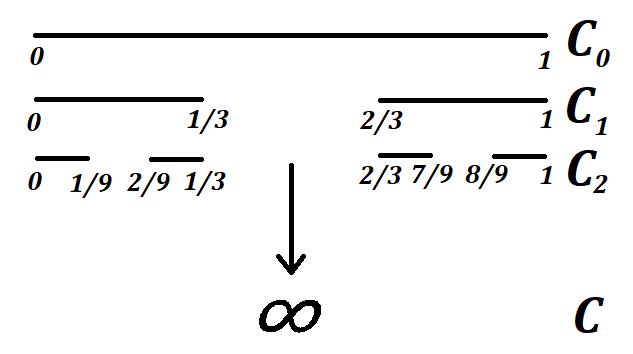
\includegraphics[scale=0.5]{pics/61_1.png}
      \end{figure}

      Определим $C_{\frac{1}{3^p}}$ как множество отрезков, получинных для $\E = \dfrac{1}{3^p}$ для крайних точек каждого отрезка из $C_p$ (они их покроют "вплотную" и по краям будет немного лишнего). На каждом шаге $p$ у нас $2^p$ отрезков
      \[\Rightarrow |C_{\frac{1}{3^p}}| = 5 \frac{2^{p-1}}{3^p} \underset{p \rightarrow \infty}{\rightarrow} 0\]
  \end{examples}

  \subsection{Критерий Лебега интегрируемости функции}

  \begin{theorem}
      Пусть $f: [a,b] \rightarrow \R$, тогда:

      $f \in R[a,b]$ $\lra$ $f$ имеет ограниченное мн-во точек разрыва и меру 0
  \end{theorem}

  \begin{examples}
      1) Функция Дирихле $\mathcal{D}(x) =
      \begin{cases}
         1, & x \in \Q\\
         0, & x \notin \Q
       \end{cases}$

      $\mathcal{D} \notin R[0,1]$. Проверим по критерию Лебега. Множество точек разрыва - $\R$, но оно не множество меры 0 (слишком много точек).

      2) Функция Римана Ф$(x) =
      \begin{cases}
         0, & x \notin \Q\\
         \frac{1}{n}, & x = \frac{m}{n} \text{ - несократимая дробь}
       \end{cases}$
      \\
      Оказывается, она интегрируема по Риману на любом отрезке. Рассмотрим [0,1]:

      a) $\forall a \in \Q$ - точка разрыва Ф:

      Ф$(a) > 0$ по определению. С другой стороны как угодно близко найдётся иррациональная точка, в которой функция принимает значение 0.

      б) $\forall a \notin \Q$ - непрерывна:

      Для произвольного $\E > 0$ рассмотрим множество $M=\{ x \in \R: f(x) \ge \E \}$.

      Никакая иррациональная точка не лежит в $M$, поскольку в иррациональных точках функция $f$ обращается в ноль.

      Если $x\in M$, тогда $x$ есть рациональное число вида $x=\frac{m}{n}$, где $m\in\mathbb{Z},\ n\in\mathbb{N}$, дробь $\frac{m}{n}$ несократима, и тогда $f(x)=\frac{1}{n} \ge \E$ и, следовательно, $n \le \frac{1}{\E}$. Из ограничения на $n$ следует, что пересечение множества $M$ и любого ограниченного интервала состоит из конечного числа точек.

      Пусть $\upalpha$ - произвольное иррациональное число. По определению $f(\upalpha)=0$. Мы можем выбрать окрестность точки $\upalpha$ так, чтобы в ней не содержалась ни одна точка множества $M$. Если же $x \notin M$, то $f(x) < \E$. Таким образом, мы нашли интервал, который требуется в определении непрерывности.
  \end{examples}

  \subsection{Что можно посмотреть ещё?}
  \begin{enumerate}
    \item Зорич В.А. «Математический анализ»
    \item Виноградов О.Л. «Математический анализ»
    \item Образовательная манга. Занимательная математика. Анализ Фурье \blacksmiley
  \end{enumerate}

\end{document}
